% !TeX program = xelatex
\documentclass{article}
\usepackage{xeCJK}
\usepackage{tikz}
\usepackage[outline]{contour}
\usepackage{graphicx}
\graphicspath{ {./} }
\setCJKmainfont{Kaiti SC}
% \setCJKmainfont{Xingkai SC}
% \setCJKmainfont{STKaiti}

\newcommand\Grid[1]{%
 \tikz[baseline=(char.base)]{%
  \draw[xstep=1ex,ystep=1ex,help lines] (-1ex,-1ex) grid (1ex,1ex);
  \draw[help lines,densely dash dot]
  (-1ex,-1ex) -- (1ex,1ex)  (-1ex,1ex) -- (1ex,-1ex);
  \node[inner sep=0pt] (char) at (0,0) {#1};
 }%
}
\pagenumbering{gobble}
\begin{document}
\begin{center}
    \Huge 春晓 \\
\end{center}
\begin{flushright}
    \huge 唐 $\bullet$ 孟浩然 \\
\end{flushright}
\begin{center}
    \Huge 春眠不觉晓 \\
    \Huge 处处闻啼鸟 \\
    \Huge 夜来风雨声 \\
    \Huge 花落知多少 \\
\end{center}
\hrule
\begin{center}
    \Huge \Grid{春}\Grid{晓} \\
\end{center}
\begin{flushright}
    \huge \Grid{唐} $\bullet$ \Grid{孟}\Grid{浩}\Grid{然} \\
\end{flushright}
\begin{center}
    \Huge \Grid{春}\Grid{眠}\Grid{不}\Grid{觉}\Grid{晓} \\
    \Huge \Grid{处}\Grid{处}\Grid{闻}\Grid{啼}\Grid{鸟} \\
    \Huge \Grid{夜}\Grid{来}\Grid{风}\Grid{雨}\Grid{声} \\
    \Huge \Grid{花}\Grid{落}\Grid{知}\Grid{多}\Grid{少} \\
\end{center}
\hrule
\begin{figure}
    \centering
    \makebox[0pt]{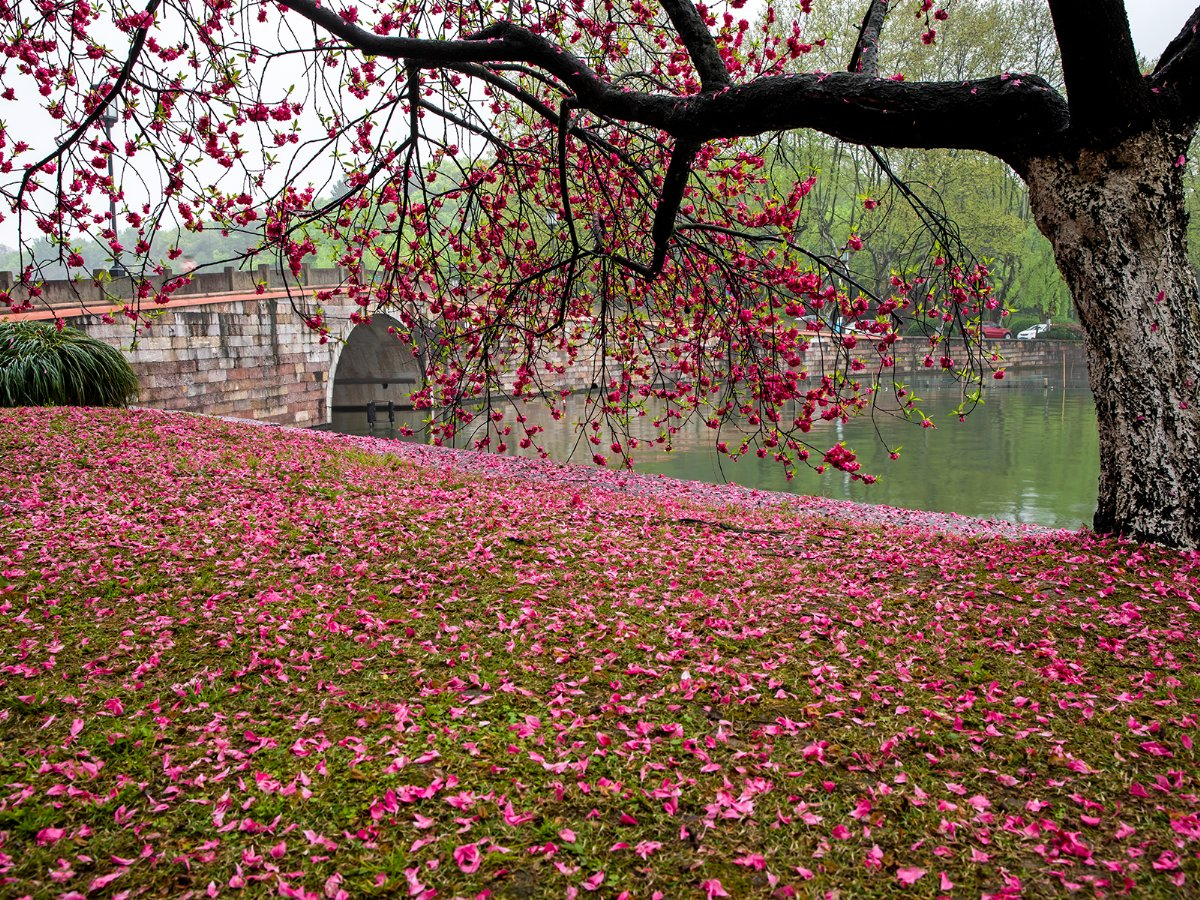
\includegraphics[width=0.9\paperwidth]{image1.jpeg}}
\end{figure}
\hrule
\begin{figure}
    \centering
    \makebox[0pt]{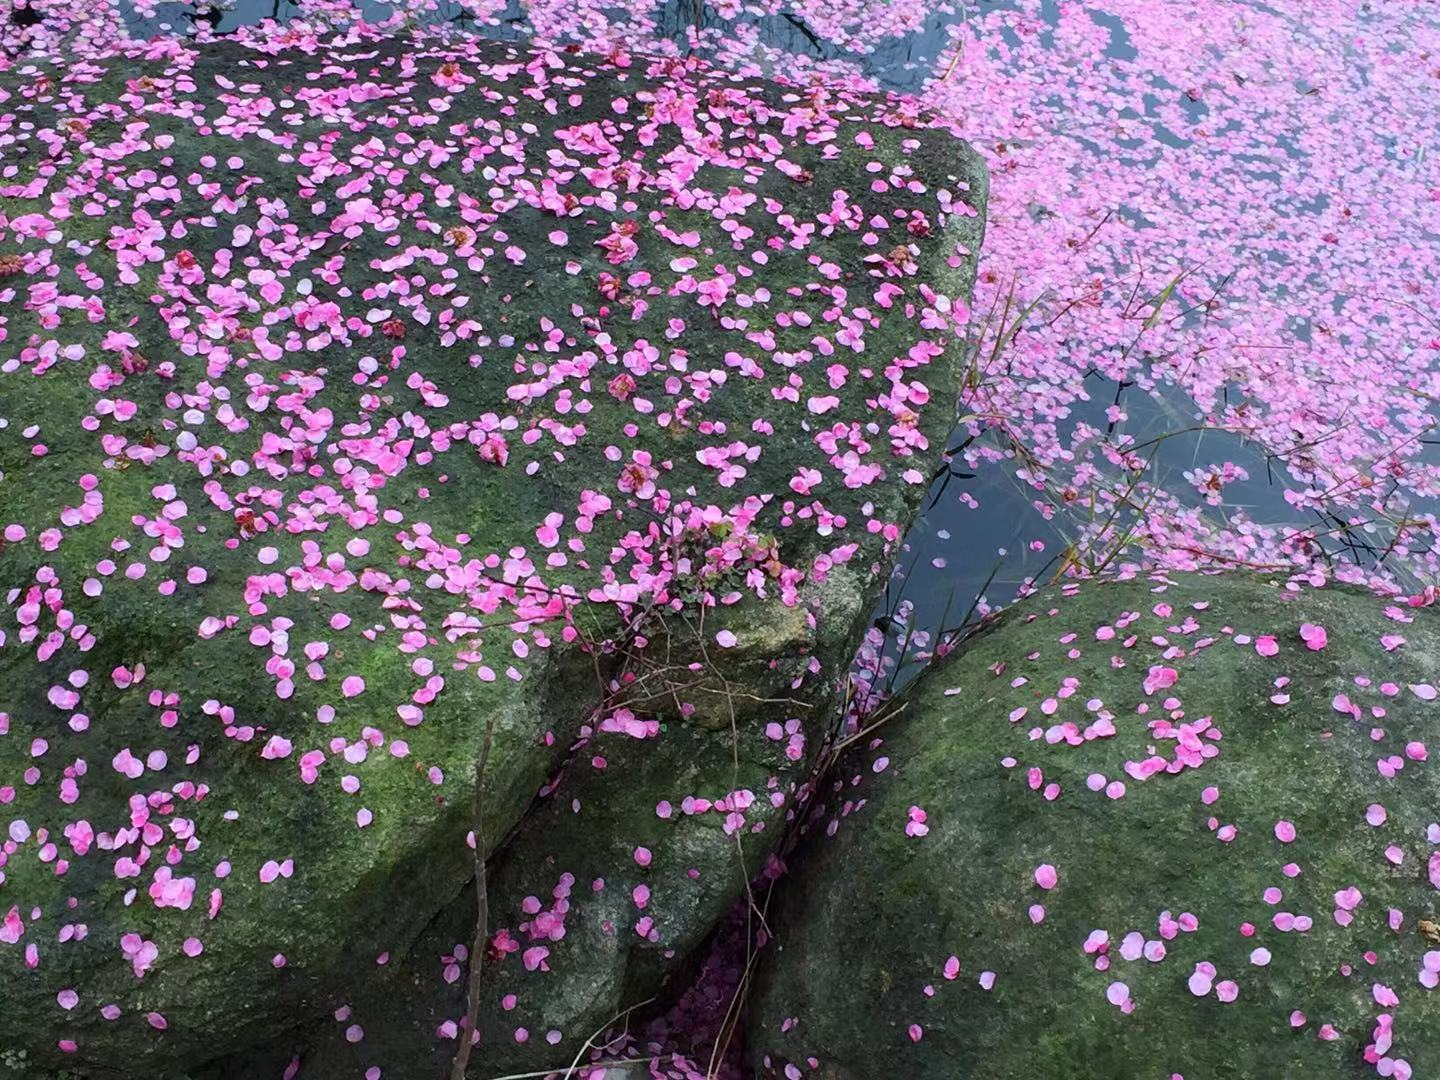
\includegraphics[width=0.9\paperwidth]{image2.jpeg}}
\end{figure}
\hrule
\begin{figure}
    \centering
    \makebox[0pt]{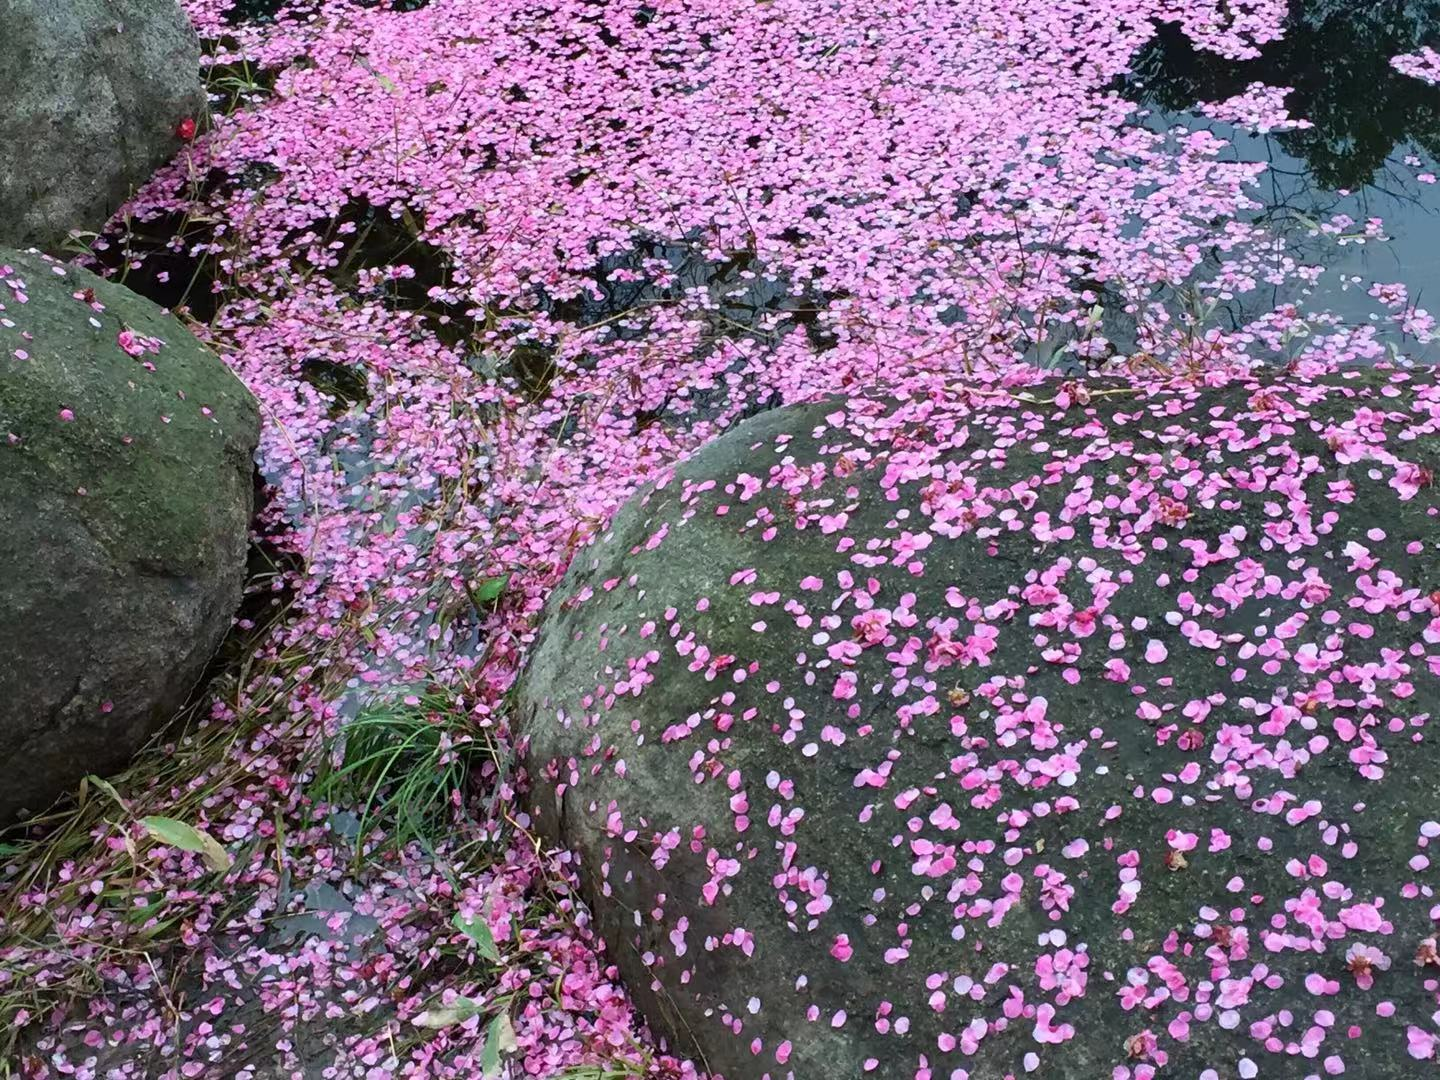
\includegraphics[width=0.9\paperwidth]{image3.jpeg}}
\end{figure}
\end{document}
